\chapter{Interfaces gráficas}

Todo programa necesita contar con algún mecanismo para recibir la
entrada y entregar la salida. Ya hemos visto dos maneras de hacer
entrada:
\begin{itemize}
\item
  entrada por teclado (\lstinline!raw_input!), y
\item
  entrada por archivo (\lstinline!for linea in archivo: ...!);
\end{itemize}
y dos maneras de hacer salida:
\begin{itemize}
\item
  salida por consola (\lstinline!print!), y
\item
  salida por archivo (\lstinline!archivo.write(...)!).
\end{itemize}

La mayoría de los programas que usamos a diario no funcionan así, sino
que tienen una \textbf{interfaz gráfica}, compuesta por ventanas,
menúes, botones y otros elementos, a través de los cuales podemos
interactuar con el programa.

Los programas con interfaces gráficas son fundamentalmente diferentes a
los programas con interfaces de texto. Los programas que hemos escrito
hasta ahora se ejecutan completamente de principio a fin, deteniéndose
sólo cuando debemos ingresar datos.

Los programas gráficos, por otra parte, realizan acciones sólo cuando
ocu\-rren ciertos eventos provocados por el usuario (como hacer clic en un
botón, o escribir algo en una casilla de texto), y el resto del tiempo
se quedan esperando que algo ocurra, sin hacer nada. El programa no
tiene control sobre cuándo debe hacer algo. Esto requiere que los
programas sean estructurados de una manera especial, que iremos
aprendiendo de a poco.

Python incluye un módulo llamado \lstinline!Tkinter! que provee todas
las funciones necesarias, que deben ser importadas al principio del
programa:
\begin{lstlisting}
from Tkinter import *
\end{lstlisting}

\section{Creación de la ventana}

El siguiente programa es la interfaz gráfica más simple que se puede
crear:
\begin{lstlisting}
from Tkinter import *
w = Tk()
w.mainloop()
\end{lstlisting}

Haga la prueba: copie este programa en el editor de texto, guárdelo y
ejecútelo. Debería aparecer una ventana vacía:

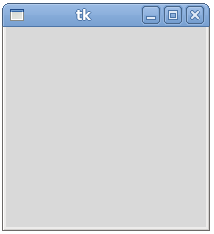
\includegraphics[scale=.5]{../diapos/programas/tkinter/capturas/01.png}

La sentencia \lstinline!w = Tk()! crea la ventana principal del
programa, y la asigna a la variable \lstinline!w!. Toda interfaz gráfica
debe tener una ventana principal en la que se irán agregando cosas. Esta
línea va al principio del programa.

La sentencia \lstinline!w.mainloop()! indica a la interfaz que debe
quedarse esperando a que el usuario haga algo. Esta línea siempre debe
ir al final del programa.

Al ejecutarlo, puede darse cuenta que el programa no termina. Esto
ocurre porque la llamada al método \lstinline!mainloop()! se «queda
pegada» esperando que algo ocurra. Esto se llama un \textbf{ciclo de
eventos}, y es simplemente un ciclo infinito que está continuamente
esperando que algo ocurra.

Todos los programas con interfaz gráfica deben seguir esta estructura:
la creación de la ventana al principio del programa y la llamada al
ciclo de eventos al final del programa.

\section{Creación de widgets}

Un \textbf{widget} es cualquier cosa que uno puede poner en una ventana.
Por ahora, veremos tres tipos de widgets sencillos, que son suficientes
para crear una interfaz gráfica funcional:

\begin{itemize}
\item
  las \textbf{etiquetas} (\lstinline!Label!) sirven para mostrar datos,
\item
  los \textbf{botones} (\lstinline!Button!) sirven para hacer que algo
  ocurra en el programa, y
\item
  los \textbf{campos de entrada} (\lstinline!Entry!) sirven para
  ingresar datos al programa.
\end{itemize}

En un programa en ejecución, estos widgets se ven así:

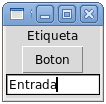
\includegraphics{../diapos/programas/tkinter/capturas/widgets.png}

El \lstinline!Entry! es análogo al \lstinline!raw_input! de los
programas de consola: sirve para que el programa reciba la entrada. El
\lstinline!Label! es análogo al \lstinline!print!: sirve para que el
programa entregue la salida.

Un botón puede ser visto como un «llamador de funciones»: cada vez que
un botón es presionado, se hace una llamada a la función asociada a ese
botón. Los botones no tienen un análogo, pues los programas de consola
se ejecutan de principio a fin inmediatamente, y por esto no necesitan
que las llamadas a las funciones sean gatilladas por el usuario.

Para agregar un widget a un programa, hay que ocupar las funciones con
los nombres de los widgets (\lstinline!Label!, \lstinline!Button! y
\lstinline!Entry!). Estas funciones reciben como primer parámetro
obligatorio la ventana que contendrá el widget. Además, tienen
parámetros opcionales que deben ser pasados usando la sintaxis de
asignación de parámetros por nombre. Por ejemplo, el parámetro
\lstinline!text! sirve para indicar cuál es el texto que aparecerá en un
botón o en una etiqueta.

Por ejemplo, la siguiente sentencia crea un botón con el texto
\lstinline!Saludar!, contenido en la ventana \lstinline!w!:

\begin{lstlisting}
b = Button(w, text='Saludar')
\end{lstlisting}

Si bien esto crea el botón y lo asigna a la variable \lstinline!b!, el
botón no es agregado a la ventana \lstinline!w! inmediatamente: lo que
hicimos fue simplemente decirle al botón cuál es su contenedor, para que
lo tenga en cuenta al momento de ser agregado. Para que esto ocurra,
debemos llamar al método \lstinline!pack!, que es una manera de decirle
al widget «empaquétate dentro de tu contenedor»:

\begin{lstlisting}
b.pack()
\end{lstlisting}

Como referencia, el programa que crea la ventana de la imagen es el
si\-guiente (¡pruébelo!):
\begin{lstlisting}
from Tkinter import *

w = Tk()

l = Label(w, text='Etiqueta')
l.pack()

b = Button(w, text='Boton')
b.pack()

e = Entry(w)
e.pack()

w.mainloop()
\end{lstlisting}



Los widgets van siendo apilados verticalmente, desde arriba hacia abajo,
en el mismo orden en que van siendo apilados. Ya veremos cómo
empaquetarlos en otras direcciones.

\section{Controladores}

Al crear un botón de la siguiente manera:
\begin{lstlisting}
b = Button(w, text='Saludar')
\end{lstlisting}
no hay ninguna acción asociada a él. Al hacer clic en el botón, nada
ocurrirá.

Para que ocurra algo al hacer clic en el botón, hay que asociarle una
acción. Un \textbf{controlador} es una función que será ejecutada al
hacer clic en un botón.

Los controladores deben ser funciones que no reciben ningún parámetro.

Por ejemplo, supongamos que queremos que el programa imprima el mensaje
\lstinline!Hola! en la consola cada vez que se haga clic en el botón que
dice «Saludar». Primero, hay que crear el controlador:
\begin{lstlisting}
def saludar():
    print 'Hola'
\end{lstlisting}

Para asociar el controlador al botón, hay que pasarlo a través del
parámetro \lstinline!command! (en inglés: «orden») al momento de crear
el botón:
\begin{lstlisting}
b = Button(w, text='Saludar', command=saludar)
\end{lstlisting}

Esta línea significa: crear el botón \lstinline!b!, contenido en la
ventana \lstinline!w!, que tenga el texto \lstinline!'Saludar'! y que al
hacer clic en él se ejecute la función \lstinline!saludar!.

El siguiente ejemplo es un programa completo que tiene dos botones: uno
para saludar y otro para salir del programa. El controlador del segundo
botón es la función \lstinline!exit!, que ya viene con Python:

\begin{lstlisting}
from Tkinter import *

def saludar():
    print 'Hola'

w = Tk()

l = Label(w, text='Hola progra')
l.pack()

b1 = Button(w, text='Saludar', command=saludar)
b1.pack()

b2 = Button(w, text='Salir', command=exit)
b2.pack()

w.mainloop()
\end{lstlisting}

El programa se ve así:

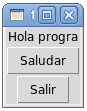
\includegraphics{../diapos/programas/tkinter/capturas/04.png}

Ejecute el programa, y pruebe lo que ocurre al hacer clic en ambos
botones.

\section{Modelos}

Mediante el uso de controladores, ya podemos hacer interfaces que hagan
algo, pero que siguen teniendo una limitación: las interfaces sólo
reaccionan a eventos que ocurren, pero no tienen memoria para recordar
información.

Un \textbf{modelo} es un dato almacenado que está asociado a la
interfaz. Usando modelos, se puede lograr que la interfaz vaya cambiando
su estado interno a medida que ocurren eventos.

En general, a la hora de crear un programa con interfaz gráfica, debemos
crear un modelo para cada dato que deba ser recordado durante el
programa.

Tkinter provee varios tipos de modelos, pero para simplificar podemos
limitarnos a usar sólo modelos de tipo string. Un modelo puede ser
creado de la siguiente manera:

\begin{lstlisting}
m = StringVar()
\end{lstlisting}

Aquí, el modelo \lstinline!m! es capaz de recordar un string

Para modificar el valor del modelo \lstinline!m!, se debe usar el método
\lstinline!set!, que recibe el valor como único parámetro:

\begin{lstlisting}
m.set('hola')
\end{lstlisting}

Para obtener el valor del modelo \lstinline!m!, se debe usar el método
\lstinline!get!, que no recibe ningún parámetro:

\begin{lstlisting}
s = m.get()
\end{lstlisting}

En este ejemplo, la variable \lstinline!s! toma el valor
\lstinline!'hola'!.

Como los modelos creados por \lstinline!StringVar! almacenan datos de
tipo string, hay que tener cuidado de hacer las conversiones apropiadas
si se desea usar datos numéricos:

\begin{lstlisting}
a = StringVar()
b = StringVar()
a.set(5)                # es convertido a string
b.set(8)                # es convertido a string
print a.get() + b.get()             # imprime 58
print int(a.get()) + int(b.get())   # imprime 13
\end{lstlisting}

Usted podría preguntarse cuál es la razón para usar modelos en vez de
usar las variables propias de Python, ---es decir, las que son creadas
mediante asignaciones--- para almacenar los datos. Los modelos tienen la
ventaja que es posible asociarlos a elementos de la interfaz que
responden automáticamente cuando el valor del modelo cambia.

Por ejemplo, podemos asociar una etiqueta a un modelo. La etiqueta
siempre mostrará en la interfaz el valor que tiene el modelo, incluso
cuando éste cambie.
El parámetro \lstinline!textvariable!
asocia el modelo a la etiqueta:

\begin{lstlisting}
x = StringVar()
l = Label(w, textvariable=x)
l.pack()
\end{lstlisting}

Cada vez que cambie el valor del modelo \lstinline!x!, el texto de la
etiqueta será actua\-li\-zado inmediatamente.

También podemos asociar un campo de entrada a un modelo. El valor
asociado al modelo siempre será el texto que está ingresado en el campo.

Para asociar un modelo a un campo de texto, también se usa el parámetro
\lstinline!textvariable!:

\begin{lstlisting}
x = StringVar()
e = Entry(w, textvariable=x)
e.pack()
\end{lstlisting}

Cuando se obtenga el valor del modelo mediante la llamada
\lstinline!x.get()!, el valor retornado será lo que el usuario haya
ingresado en el campo hasta ese momento.

\section{Resumen}

Para diseñar un programa que tiene una interfaz gráfica, hay tres
elementos importantes que hay que tener en consideración.

\begin{enumerate}
\item
  Los elementos que componen la interfaz (la \textbf{vista} del programa).
\item
  Los \textbf{modelos} que mantienen el estado de la interfaz en todo
  momento.
\item
  Los \textbf{controladores} que reaccionan a eventos del usuario.
\end{enumerate}

Los controladores pueden interactuar con los modelos mediante sus
métodos \lstinline!get! y \lstinline[language={}]!set!. Los cambios en los modelos
pueden verse reflejados en la vista.
